\documentclass[a4paper]{tufte-handout}

% ams
\usepackage{amssymb,amsmath}

\usepackage{ifxetex,ifluatex}
\usepackage{fixltx2e} % provides \textsubscript
\ifnum 0\ifxetex 1\fi\ifluatex 1\fi=0 % if pdftex
  \usepackage[T1]{fontenc}
  \usepackage[utf8]{inputenc}
\else % if luatex or xelatex
  \makeatletter
  \@ifpackageloaded{fontspec}{}{\usepackage{fontspec}}
  \makeatother
  \defaultfontfeatures{Ligatures=TeX,Scale=MatchLowercase}
  \makeatletter
  \@ifpackageloaded{soul}{
     \renewcommand\allcapsspacing[1]{{\addfontfeature{LetterSpace=15}#1}}
     \renewcommand\smallcapsspacing[1]{{\addfontfeature{LetterSpace=10}#1}}
   }{}
  \makeatother

\fi

% graphix
\usepackage{graphicx}
\setkeys{Gin}{width=\linewidth,totalheight=\textheight,keepaspectratio}

% booktabs
\usepackage{booktabs}

% url
\usepackage{url}

% hyperref
\usepackage{hyperref}

% units.
\usepackage{units}


\setcounter{secnumdepth}{-1}

% citations
\usepackage{natbib}
\bibliographystyle{plainnat}


% pandoc syntax highlighting
\usepackage{color}
\usepackage{fancyvrb}
\newcommand{\VerbBar}{|}
\newcommand{\VERB}{\Verb[commandchars=\\\{\}]}
\DefineVerbatimEnvironment{Highlighting}{Verbatim}{commandchars=\\\{\}}
% Add ',fontsize=\small' for more characters per line
\newenvironment{Shaded}{}{}
\newcommand{\AlertTok}[1]{\textcolor[rgb]{1.00,0.00,0.00}{\textbf{#1}}}
\newcommand{\AnnotationTok}[1]{\textcolor[rgb]{0.38,0.63,0.69}{\textbf{\textit{#1}}}}
\newcommand{\AttributeTok}[1]{\textcolor[rgb]{0.49,0.56,0.16}{#1}}
\newcommand{\BaseNTok}[1]{\textcolor[rgb]{0.25,0.63,0.44}{#1}}
\newcommand{\BuiltInTok}[1]{#1}
\newcommand{\CharTok}[1]{\textcolor[rgb]{0.25,0.44,0.63}{#1}}
\newcommand{\CommentTok}[1]{\textcolor[rgb]{0.38,0.63,0.69}{\textit{#1}}}
\newcommand{\CommentVarTok}[1]{\textcolor[rgb]{0.38,0.63,0.69}{\textbf{\textit{#1}}}}
\newcommand{\ConstantTok}[1]{\textcolor[rgb]{0.53,0.00,0.00}{#1}}
\newcommand{\ControlFlowTok}[1]{\textcolor[rgb]{0.00,0.44,0.13}{\textbf{#1}}}
\newcommand{\DataTypeTok}[1]{\textcolor[rgb]{0.56,0.13,0.00}{#1}}
\newcommand{\DecValTok}[1]{\textcolor[rgb]{0.25,0.63,0.44}{#1}}
\newcommand{\DocumentationTok}[1]{\textcolor[rgb]{0.73,0.13,0.13}{\textit{#1}}}
\newcommand{\ErrorTok}[1]{\textcolor[rgb]{1.00,0.00,0.00}{\textbf{#1}}}
\newcommand{\ExtensionTok}[1]{#1}
\newcommand{\FloatTok}[1]{\textcolor[rgb]{0.25,0.63,0.44}{#1}}
\newcommand{\FunctionTok}[1]{\textcolor[rgb]{0.02,0.16,0.49}{#1}}
\newcommand{\ImportTok}[1]{#1}
\newcommand{\InformationTok}[1]{\textcolor[rgb]{0.38,0.63,0.69}{\textbf{\textit{#1}}}}
\newcommand{\KeywordTok}[1]{\textcolor[rgb]{0.00,0.44,0.13}{\textbf{#1}}}
\newcommand{\NormalTok}[1]{#1}
\newcommand{\OperatorTok}[1]{\textcolor[rgb]{0.40,0.40,0.40}{#1}}
\newcommand{\OtherTok}[1]{\textcolor[rgb]{0.00,0.44,0.13}{#1}}
\newcommand{\PreprocessorTok}[1]{\textcolor[rgb]{0.74,0.48,0.00}{#1}}
\newcommand{\RegionMarkerTok}[1]{#1}
\newcommand{\SpecialCharTok}[1]{\textcolor[rgb]{0.25,0.44,0.63}{#1}}
\newcommand{\SpecialStringTok}[1]{\textcolor[rgb]{0.73,0.40,0.53}{#1}}
\newcommand{\StringTok}[1]{\textcolor[rgb]{0.25,0.44,0.63}{#1}}
\newcommand{\VariableTok}[1]{\textcolor[rgb]{0.10,0.09,0.49}{#1}}
\newcommand{\VerbatimStringTok}[1]{\textcolor[rgb]{0.25,0.44,0.63}{#1}}
\newcommand{\WarningTok}[1]{\textcolor[rgb]{0.38,0.63,0.69}{\textbf{\textit{#1}}}}

% longtable

% multiplecol
\usepackage{multicol}

% strikeout
\usepackage[normalem]{ulem}

% morefloats
\usepackage{morefloats}


% tightlist macro required by pandoc >= 1.14
\providecommand{\tightlist}{%
  \setlength{\itemsep}{0pt}\setlength{\parskip}{0pt}}

% title / author / date
\title[分散の加法性を視覚的に理解する(その4)]{分散の加法性を視覚的に理解する(その4)}
\author{Sampo Suzuki, CC 4.0 BY-NC-SA}
\date{2021-06-05}

% --- 参考資料 ----------------------------------------------------------------
% http://ctan.math.illinois.edu/language/japanese/zxjafont/zxjafont.pdf
% https://github.com/Gedevan-Aleksizde/Japan.R2019/blob/master/latex/preamble.tex
% https://teastat.blogspot.com/2019/01/bookdown.html

% --- Packages ----------------------------------------------------------------
% 日本語とtufte, kableExtraを使うために必要なTeXパッケージ指定
% \usepackage[pdfbox,tombo]{gentombow}    % トンボを設定する場合は有効にする
\usepackage{ifthen}                     % 条件分岐用 \ifthenelse{条件}{T}{F}
\usepackage{booktabs}                   % ここからkableExtra用パッケージ
\usepackage{longtable}                  % 
\usepackage{array}                      % 
\usepackage{multirow}                   % 
\usepackage{wrapfig}                    % 
\usepackage{float}                      % 
\usepackage{colortbl}                   % 
\usepackage{pdflscape}                  % 
\usepackage{tabu}                       % 
\usepackage{threeparttable}             % 
\usepackage{threeparttablex}            % 
\usepackage[normalem]{ulem}             % 
\usepackage{inputenc}                   % 
\usepackage{makecell}                   % 
\usepackage{xcolor}                     % ここまでkableExtra用
\usepackage{amsmath}                    % 
\usepackage{fontawesome5}               % fontawesomeを使うために必要
\usepackage{subfig}                     % 複数の図を並べる際に必要(古い?)
% \usepackage{subcaption}                 % 同上(新しい?)
\usepackage{zxjatype}                   % 日本語処理に必要
% \usepackage{xeCJK}                      % zxjatypeを読み込むと一緒に読み込まれる
\usepackage[noto]{zxjafont}             % Linux環境用
% \usepackage[haranoaji]{zxjafont}        % Windows環境用
% \usepackage[hiragino-pro]{zxjafont}     % macOS環境用(おそらく、駄目ならNotoで)
\usepackage{pxrubrica}                  % ルビ用
\usepackage{hyperref}                   % ハイパーリンク用必要?
% 以下のパッケージについては下記サイトを参照方
% http://www.yamamo10.jp/yamamoto/comp/latex/make_doc/box/box.php
% \usepackage{ascmac}                     % 別行で文書を囲む場合
% \usepackage{fancybox}                   % 行中で文書を囲む場合 fancybx ではない
% \usepackage{fancyhdr}                   % ヘッダー用

% https://ja.wikibooks.org/wiki/TeX/LaTeX%E5%85%A5%E9%96%80
% https://teastat.blogspot.com/2019/01/bookdown.html
\usepackage{booktabs}
\usepackage{longtable}
\usepackage{array}
\usepackage{multirow}
\usepackage{wrapfig}
\usepackage{float}
\usepackage{colortbl}
\usepackage{pdflscape}
\usepackage{tabu}
\usepackage{threeparttable}
\usepackage{threeparttablex}
\usepackage[normalem]{ulem}
\usepackage{makecell}
\usepackage{xcolor}

\begin{document}

\maketitle

\begin{abstract}
\noindent  正規分布とは異なる分布でも分散の加法性が成り立つことを確認します。
\end{abstract}



\hypertarget{tux5206ux5e03ux306eux5834ux5408}{%
\section{\texorpdfstring{\textbf{t分布の場合}}{t分布の場合}}\label{tux5206ux5e03ux306eux5834ux5408}}

 自由度\(df = 1\)と\(df = 5\)のt分布の分散を以下の関数で計算します。

\begin{Shaded}
\begin{Highlighting}[numbers=left,,]
\NormalTok{ft }\OtherTok{\textless{}{-}} \ControlFlowTok{function}\NormalTok{(}\AttributeTok{i =} \ConstantTok{NA}\NormalTok{, }\AttributeTok{n =} \DecValTok{5000000}\NormalTok{, }\AttributeTok{num =} \DecValTok{2}\NormalTok{) \{}
\NormalTok{  x }\OtherTok{\textless{}{-}} \FunctionTok{rt}\NormalTok{(}\AttributeTok{n =}\NormalTok{ n, }\AttributeTok{df =} \DecValTok{1}\NormalTok{)}
\NormalTok{  y }\OtherTok{\textless{}{-}} \FunctionTok{rt}\NormalTok{(}\AttributeTok{n =}\NormalTok{ n, }\AttributeTok{df =} \DecValTok{5}\NormalTok{)}
\NormalTok{  df }\OtherTok{\textless{}{-}} \FunctionTok{data.frame}\NormalTok{(}\AttributeTok{no =}\NormalTok{ i,}
                   \AttributeTok{var.x =} \FunctionTok{var}\NormalTok{(x), }\AttributeTok{var.y =} \FunctionTok{var}\NormalTok{(y),}
                   \AttributeTok{var.xy =} \FunctionTok{var}\NormalTok{((x }\SpecialCharTok{+}\NormalTok{ y) }\SpecialCharTok{/}\NormalTok{ num), }\AttributeTok{var.sum =}\NormalTok{ (}\FunctionTok{var}\NormalTok{(x }\SpecialCharTok{/}\NormalTok{ num) }\SpecialCharTok{+} \FunctionTok{var}\NormalTok{(y }\SpecialCharTok{/}\NormalTok{ num)),}
                   \AttributeTok{cov2 =} \FunctionTok{cov}\NormalTok{(x }\SpecialCharTok{/}\NormalTok{ num, y }\SpecialCharTok{/}\NormalTok{ num) }\SpecialCharTok{*} \DecValTok{2}\NormalTok{)}
\NormalTok{  df }\OtherTok{\textless{}{-}} \FunctionTok{cor.test}\NormalTok{(x, y) }\SpecialCharTok{\%\textgreater{}\%}\NormalTok{ broom}\SpecialCharTok{::}\FunctionTok{tidy}\NormalTok{() }\SpecialCharTok{\%\textgreater{}\%}\NormalTok{ dplyr}\SpecialCharTok{::}\FunctionTok{bind\_cols}\NormalTok{(df)}
  \FunctionTok{return}\NormalTok{(df)}
\NormalTok{\}}
\end{Highlighting}
\end{Shaded}

\[\mbox{加法1:}var.xy = var(\frac{x + y}{2}), \mbox{加法2:}var.sum = var(\frac{x}{2}) + var(\frac{y}{2})\]

\begin{figure}

{\centering \subfloat[$df = 1$\label{fig:unnamed-chunk-2-1}]{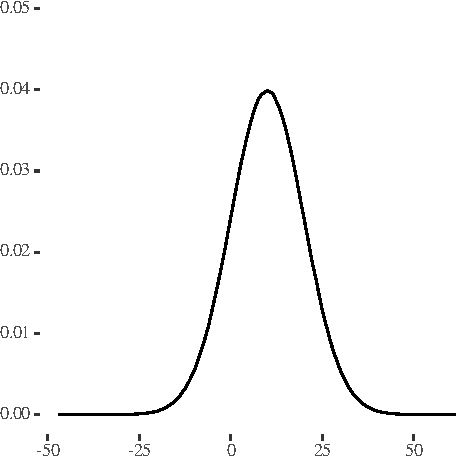
\includegraphics[width=0.4\linewidth]{AdditivityOfVariance4th_files/figure-latex/unnamed-chunk-2-1} }\subfloat[$df = 5$\label{fig:unnamed-chunk-2-2}]{\includegraphics[width=0.4\linewidth]{AdditivityOfVariance4th_files/figure-latex/unnamed-chunk-2-2} }

}

\caption[分散を加算する二種類のt分布]{分散を加算する二種類のt分布}\label{fig:unnamed-chunk-2}
\end{figure}

\begin{table}

\caption{\label{tab:unnamed-chunk-4}計算結果}
\centering
\resizebox{\linewidth}{!}{
\begin{tabular}[t]{rrrrrrrrrr}
\toprule
No & 相関係数 & p値 & 標本x & 標本y & 加法1 & 加法2 & 差異 & 加法1/加法2 & cov2\\
\midrule
\cellcolor{gray!6}{1} & \cellcolor{gray!6}{-0.0001503} & \cellcolor{gray!6}{0.7367569} & \cellcolor{gray!6}{3756872} & \cellcolor{gray!6}{1.668392} & \cellcolor{gray!6}{939218.2} & \cellcolor{gray!6}{939218.4} & \cellcolor{gray!6}{-0.1881836} & \cellcolor{gray!6}{0.9999998} & \cellcolor{gray!6}{-0.1881836}\\
2 & -0.0009528 & 0.0331366 & 5921163 & 1.665188 & 1480289.7 & 1480291.1 & -1.4958439 & 0.9999990 & -1.4958439\\
\cellcolor{gray!6}{3} & \cellcolor{gray!6}{-0.0001065} & \cellcolor{gray!6}{0.8117592} & \cellcolor{gray!6}{3170503} & \cellcolor{gray!6}{1.665145} & \cellcolor{gray!6}{792626.1} & \cellcolor{gray!6}{792626.2} & \cellcolor{gray!6}{-0.1223598} & \cellcolor{gray!6}{0.9999998} & \cellcolor{gray!6}{-0.1223598}\\
4 & 0.0001363 & 0.7605916 & 234538469 & 1.668358 & 58634619.0 & 58634617.6 & 1.3477671 & 1.0000000 & 1.3477671\\
\cellcolor{gray!6}{5} & \cellcolor{gray!6}{-0.0003846} & \cellcolor{gray!6}{0.3898150} & \cellcolor{gray!6}{21328947} & \cellcolor{gray!6}{1.667404} & \cellcolor{gray!6}{5332236.1} & \cellcolor{gray!6}{5332237.2} & \cellcolor{gray!6}{-1.1467396} & \cellcolor{gray!6}{0.9999998} & \cellcolor{gray!6}{-1.1467396}\\
\addlinespace
6 & 0.0000707 & 0.8744723 & 2824118 & 1.670452 & 706030.1 & 706030.0 & 0.0767267 & 1.0000001 & 0.0767267\\
\cellcolor{gray!6}{7} & \cellcolor{gray!6}{-0.0003141} & \cellcolor{gray!6}{0.4824975} & \cellcolor{gray!6}{31822527} & \cellcolor{gray!6}{1.667388} & \cellcolor{gray!6}{7955631.0} & \cellcolor{gray!6}{7955632.1} & \cellcolor{gray!6}{-1.1438998} & \cellcolor{gray!6}{0.9999999} & \cellcolor{gray!6}{-1.1438998}\\
8 & -0.0001649 & 0.7124014 & 29039432 & 1.665014 & 7259857.9 & 7259858.5 & -0.5731684 & 0.9999999 & -0.5731684\\
\cellcolor{gray!6}{9} & \cellcolor{gray!6}{-0.0001918} & \cellcolor{gray!6}{0.6680222} & \cellcolor{gray!6}{16324840} & \cellcolor{gray!6}{1.667192} & \cellcolor{gray!6}{4081210.0} & \cellcolor{gray!6}{4081210.5} & \cellcolor{gray!6}{-0.5002902} & \cellcolor{gray!6}{0.9999999} & \cellcolor{gray!6}{-0.5002902}\\
10 & -0.0006548 & 0.1431528 & 1649851 & 1.668310 & 412462.5 & 412463.0 & -0.5431646 & 0.9999987 & -0.5431646\\
\addlinespace
\cellcolor{gray!6}{11} & \cellcolor{gray!6}{-0.0004414} & \cellcolor{gray!6}{0.3235916} & \cellcolor{gray!6}{39759746} & \cellcolor{gray!6}{1.667619} & \cellcolor{gray!6}{9939935.2} & \cellcolor{gray!6}{9939937.0} & \cellcolor{gray!6}{-1.7972904} & \cellcolor{gray!6}{0.9999998} & \cellcolor{gray!6}{-1.7972904}\\
12 & 0.0005128 & 0.2515537 & 163643080 & 1.664719 & 40910774.7 & 40910770.5 & 4.2316546 & 1.0000001 & 4.2316546\\
\cellcolor{gray!6}{13} & \cellcolor{gray!6}{-0.0004253} & \cellcolor{gray!6}{0.3416042} & \cellcolor{gray!6}{11220099} & \cellcolor{gray!6}{1.666779} & \cellcolor{gray!6}{2805024.3} & \cellcolor{gray!6}{2805025.2} & \cellcolor{gray!6}{-0.9196087} & \cellcolor{gray!6}{0.9999997} & \cellcolor{gray!6}{-0.9196087}\\
14 & -0.0001211 & 0.7865968 & 61321544 & 1.666002 & 15330385.8 & 15330386.4 & -0.6118848 & 1.0000000 & -0.6118848\\
\cellcolor{gray!6}{15} & \cellcolor{gray!6}{-0.0000186} & \cellcolor{gray!6}{0.9668654} & \cellcolor{gray!6}{431531} & \cellcolor{gray!6}{1.665694} & \cellcolor{gray!6}{107883.2} & \cellcolor{gray!6}{107883.2} & \cellcolor{gray!6}{-0.0078751} & \cellcolor{gray!6}{0.9999999} & \cellcolor{gray!6}{-0.0078751}\\
\addlinespace
16 & 0.0003024 & 0.4988689 & 7363469 & 1.664964 & 1840868.3 & 1840867.8 & 0.5294797 & 1.0000003 & 0.5294797\\
\cellcolor{gray!6}{17} & \cellcolor{gray!6}{-0.0000513} & \cellcolor{gray!6}{0.9087598} & \cellcolor{gray!6}{611103876} & \cellcolor{gray!6}{1.666259} & \cellcolor{gray!6}{152775968.7} & \cellcolor{gray!6}{152775969.5} & \cellcolor{gray!6}{-0.8177302} & \cellcolor{gray!6}{1.0000000} & \cellcolor{gray!6}{-0.8177302}\\
18 & -0.0002512 & 0.5743927 & 1643759 & 1.666420 & 410939.9 & 410940.1 & -0.2078351 & 0.9999995 & -0.2078351\\
\cellcolor{gray!6}{19} & \cellcolor{gray!6}{0.0000852} & \cellcolor{gray!6}{0.8489663} & \cellcolor{gray!6}{2205786} & \cellcolor{gray!6}{1.668551} & \cellcolor{gray!6}{551446.9} & \cellcolor{gray!6}{551446.9} & \cellcolor{gray!6}{0.0816938} & \cellcolor{gray!6}{1.0000001} & \cellcolor{gray!6}{0.0816938}\\
20 & 0.0000339 & 0.9395056 & 471213880 & 1.669165 & 117803471.0 & 117803470.5 & 0.4759216 & 1.0000000 & 0.4759216\\
\bottomrule
\end{tabular}}
\end{table}

\newpage

\hypertarget{chi2ux5206ux5e03ux306eux5834ux5408}{%
\section{\texorpdfstring{\textbf{\(\chi^2\)分布の場合}}{\textbackslash chi\^{}2分布の場合}}\label{chi2ux5206ux5e03ux306eux5834ux5408}}

 自由度\(df = 1\)と\(df = 3\)の\(\chi^2\)分布の分散を以下の関数で計算します。

\begin{Shaded}
\begin{Highlighting}[numbers=left,,]
\NormalTok{fchisq }\OtherTok{\textless{}{-}} \ControlFlowTok{function}\NormalTok{(}\AttributeTok{i =} \ConstantTok{NA}\NormalTok{, }\AttributeTok{n =} \DecValTok{5000000}\NormalTok{, }\AttributeTok{num =} \DecValTok{2}\NormalTok{) \{}
\NormalTok{  x }\OtherTok{\textless{}{-}} \FunctionTok{rchisq}\NormalTok{(}\AttributeTok{n =}\NormalTok{ n, }\AttributeTok{df =} \DecValTok{1}\NormalTok{)}
\NormalTok{  y }\OtherTok{\textless{}{-}} \FunctionTok{rchisq}\NormalTok{(}\AttributeTok{n =}\NormalTok{ n, }\AttributeTok{df =} \DecValTok{3}\NormalTok{)}
\NormalTok{  df }\OtherTok{\textless{}{-}} \FunctionTok{data.frame}\NormalTok{(}\AttributeTok{no =}\NormalTok{ i,}
                   \AttributeTok{var.x =} \FunctionTok{var}\NormalTok{(x), }\AttributeTok{var.y =} \FunctionTok{var}\NormalTok{(y),}
                   \AttributeTok{var.xy =} \FunctionTok{var}\NormalTok{((x }\SpecialCharTok{+}\NormalTok{ y) }\SpecialCharTok{/}\NormalTok{ num), }\AttributeTok{var.sum =}\NormalTok{ (}\FunctionTok{var}\NormalTok{(x }\SpecialCharTok{/}\NormalTok{ num) }\SpecialCharTok{+} \FunctionTok{var}\NormalTok{(y }\SpecialCharTok{/}\NormalTok{ num)),}
                   \AttributeTok{cov2 =} \FunctionTok{cov}\NormalTok{(x }\SpecialCharTok{/}\NormalTok{ num, y }\SpecialCharTok{/}\NormalTok{ num) }\SpecialCharTok{*} \DecValTok{2}\NormalTok{)}
\NormalTok{  df }\OtherTok{\textless{}{-}} \FunctionTok{cor.test}\NormalTok{(x, y) }\SpecialCharTok{\%\textgreater{}\%}\NormalTok{ broom}\SpecialCharTok{::}\FunctionTok{tidy}\NormalTok{() }\SpecialCharTok{\%\textgreater{}\%}\NormalTok{ dplyr}\SpecialCharTok{::}\FunctionTok{bind\_cols}\NormalTok{(df)}
  \FunctionTok{return}\NormalTok{(df)}
\NormalTok{\}}
\end{Highlighting}
\end{Shaded}

\[\mbox{加法1:}var.xy = var(\frac{x + y}{2}), \mbox{加法2:}var.sum = var(\frac{x}{2}) + var(\frac{y}{2})\]

\begin{figure}

{\centering \subfloat[$df = 1$\label{fig:unnamed-chunk-6-1}]{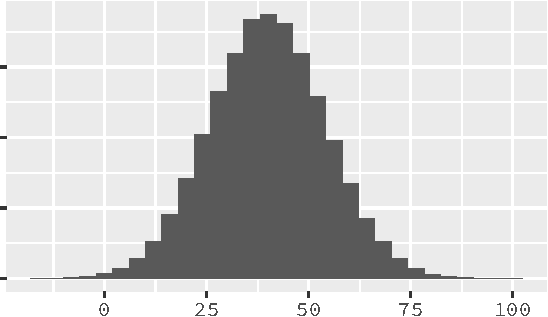
\includegraphics[width=0.4\linewidth]{AdditivityOfVariance4th_files/figure-latex/unnamed-chunk-6-1} }\subfloat[$df = 3$\label{fig:unnamed-chunk-6-2}]{\includegraphics[width=0.4\linewidth]{AdditivityOfVariance4th_files/figure-latex/unnamed-chunk-6-2} }

}

\caption[分散を加算する二種類の$\chi^2$分布]{分散を加算する二種類の$\chi^2$分布}\label{fig:unnamed-chunk-6}
\end{figure}

\begin{table}

\caption{\label{tab:unnamed-chunk-7}計算結果}
\centering
\resizebox{\linewidth}{!}{
\begin{tabular}[t]{rrrrrrrrrr}
\toprule
No & 相関係数 & p値 & 標本x & 標本y & 加法1 & 加法2 & 差異 & 加法1/加法2 & cov2\\
\midrule
\cellcolor{gray!6}{1} & \cellcolor{gray!6}{-0.0001503} & \cellcolor{gray!6}{0.7367569} & \cellcolor{gray!6}{3756872} & \cellcolor{gray!6}{1.668392} & \cellcolor{gray!6}{939218.2} & \cellcolor{gray!6}{939218.4} & \cellcolor{gray!6}{-0.1881836} & \cellcolor{gray!6}{0.9999998} & \cellcolor{gray!6}{-0.1881836}\\
2 & -0.0009528 & 0.0331366 & 5921163 & 1.665188 & 1480289.7 & 1480291.1 & -1.4958439 & 0.9999990 & -1.4958439\\
\cellcolor{gray!6}{3} & \cellcolor{gray!6}{-0.0001065} & \cellcolor{gray!6}{0.8117592} & \cellcolor{gray!6}{3170503} & \cellcolor{gray!6}{1.665145} & \cellcolor{gray!6}{792626.1} & \cellcolor{gray!6}{792626.2} & \cellcolor{gray!6}{-0.1223598} & \cellcolor{gray!6}{0.9999998} & \cellcolor{gray!6}{-0.1223598}\\
4 & 0.0001363 & 0.7605916 & 234538469 & 1.668358 & 58634619.0 & 58634617.6 & 1.3477671 & 1.0000000 & 1.3477671\\
\cellcolor{gray!6}{5} & \cellcolor{gray!6}{-0.0003846} & \cellcolor{gray!6}{0.3898150} & \cellcolor{gray!6}{21328947} & \cellcolor{gray!6}{1.667404} & \cellcolor{gray!6}{5332236.1} & \cellcolor{gray!6}{5332237.2} & \cellcolor{gray!6}{-1.1467396} & \cellcolor{gray!6}{0.9999998} & \cellcolor{gray!6}{-1.1467396}\\
\addlinespace
6 & 0.0000707 & 0.8744723 & 2824118 & 1.670452 & 706030.1 & 706030.0 & 0.0767267 & 1.0000001 & 0.0767267\\
\cellcolor{gray!6}{7} & \cellcolor{gray!6}{-0.0003141} & \cellcolor{gray!6}{0.4824975} & \cellcolor{gray!6}{31822527} & \cellcolor{gray!6}{1.667388} & \cellcolor{gray!6}{7955631.0} & \cellcolor{gray!6}{7955632.1} & \cellcolor{gray!6}{-1.1438998} & \cellcolor{gray!6}{0.9999999} & \cellcolor{gray!6}{-1.1438998}\\
8 & -0.0001649 & 0.7124014 & 29039432 & 1.665014 & 7259857.9 & 7259858.5 & -0.5731684 & 0.9999999 & -0.5731684\\
\cellcolor{gray!6}{9} & \cellcolor{gray!6}{-0.0001918} & \cellcolor{gray!6}{0.6680222} & \cellcolor{gray!6}{16324840} & \cellcolor{gray!6}{1.667192} & \cellcolor{gray!6}{4081210.0} & \cellcolor{gray!6}{4081210.5} & \cellcolor{gray!6}{-0.5002902} & \cellcolor{gray!6}{0.9999999} & \cellcolor{gray!6}{-0.5002902}\\
10 & -0.0006548 & 0.1431528 & 1649851 & 1.668310 & 412462.5 & 412463.0 & -0.5431646 & 0.9999987 & -0.5431646\\
\addlinespace
\cellcolor{gray!6}{11} & \cellcolor{gray!6}{-0.0004414} & \cellcolor{gray!6}{0.3235916} & \cellcolor{gray!6}{39759746} & \cellcolor{gray!6}{1.667619} & \cellcolor{gray!6}{9939935.2} & \cellcolor{gray!6}{9939937.0} & \cellcolor{gray!6}{-1.7972904} & \cellcolor{gray!6}{0.9999998} & \cellcolor{gray!6}{-1.7972904}\\
12 & 0.0005128 & 0.2515537 & 163643080 & 1.664719 & 40910774.7 & 40910770.5 & 4.2316546 & 1.0000001 & 4.2316546\\
\cellcolor{gray!6}{13} & \cellcolor{gray!6}{-0.0004253} & \cellcolor{gray!6}{0.3416042} & \cellcolor{gray!6}{11220099} & \cellcolor{gray!6}{1.666779} & \cellcolor{gray!6}{2805024.3} & \cellcolor{gray!6}{2805025.2} & \cellcolor{gray!6}{-0.9196087} & \cellcolor{gray!6}{0.9999997} & \cellcolor{gray!6}{-0.9196087}\\
14 & -0.0001211 & 0.7865968 & 61321544 & 1.666002 & 15330385.8 & 15330386.4 & -0.6118848 & 1.0000000 & -0.6118848\\
\cellcolor{gray!6}{15} & \cellcolor{gray!6}{-0.0000186} & \cellcolor{gray!6}{0.9668654} & \cellcolor{gray!6}{431531} & \cellcolor{gray!6}{1.665694} & \cellcolor{gray!6}{107883.2} & \cellcolor{gray!6}{107883.2} & \cellcolor{gray!6}{-0.0078751} & \cellcolor{gray!6}{0.9999999} & \cellcolor{gray!6}{-0.0078751}\\
\addlinespace
16 & 0.0003024 & 0.4988689 & 7363469 & 1.664964 & 1840868.3 & 1840867.8 & 0.5294797 & 1.0000003 & 0.5294797\\
\cellcolor{gray!6}{17} & \cellcolor{gray!6}{-0.0000513} & \cellcolor{gray!6}{0.9087598} & \cellcolor{gray!6}{611103876} & \cellcolor{gray!6}{1.666259} & \cellcolor{gray!6}{152775968.7} & \cellcolor{gray!6}{152775969.5} & \cellcolor{gray!6}{-0.8177302} & \cellcolor{gray!6}{1.0000000} & \cellcolor{gray!6}{-0.8177302}\\
18 & -0.0002512 & 0.5743927 & 1643759 & 1.666420 & 410939.9 & 410940.1 & -0.2078351 & 0.9999995 & -0.2078351\\
\cellcolor{gray!6}{19} & \cellcolor{gray!6}{0.0000852} & \cellcolor{gray!6}{0.8489663} & \cellcolor{gray!6}{2205786} & \cellcolor{gray!6}{1.668551} & \cellcolor{gray!6}{551446.9} & \cellcolor{gray!6}{551446.9} & \cellcolor{gray!6}{0.0816938} & \cellcolor{gray!6}{1.0000001} & \cellcolor{gray!6}{0.0816938}\\
20 & 0.0000339 & 0.9395056 & 471213880 & 1.669165 & 117803471.0 & 117803470.5 & 0.4759216 & 1.0000000 & 0.4759216\\
\bottomrule
\end{tabular}}
\end{table}

\newpage

\hypertarget{fux5206ux5e03ux306eux5834ux5408}{%
\section{\texorpdfstring{\textbf{F分布の場合}}{F分布の場合}}\label{fux5206ux5e03ux306eux5834ux5408}}

 自由度\(df_1 = 3, df_2 = 6\)と\(df_1 = 9, df_2 = 3\)のF分布の分散を以下の関数で計算します。

\begin{Shaded}
\begin{Highlighting}[numbers=left,,]
\NormalTok{ff }\OtherTok{\textless{}{-}} \ControlFlowTok{function}\NormalTok{(}\AttributeTok{i =} \ConstantTok{NA}\NormalTok{, }\AttributeTok{n =} \DecValTok{5000000}\NormalTok{, }\AttributeTok{num =} \DecValTok{2}\NormalTok{) \{}
\NormalTok{  x }\OtherTok{\textless{}{-}} \FunctionTok{rf}\NormalTok{(}\AttributeTok{n =}\NormalTok{ n, }\AttributeTok{df1 =} \DecValTok{3}\NormalTok{, }\AttributeTok{df2 =} \DecValTok{6}\NormalTok{)}
\NormalTok{  y }\OtherTok{\textless{}{-}} \FunctionTok{rf}\NormalTok{(}\AttributeTok{n =}\NormalTok{ n, }\AttributeTok{df1 =} \DecValTok{9}\NormalTok{, }\AttributeTok{df2 =} \DecValTok{3}\NormalTok{)}
\NormalTok{  df }\OtherTok{\textless{}{-}} \FunctionTok{data.frame}\NormalTok{(}\AttributeTok{no =}\NormalTok{ i,}
                   \AttributeTok{var.x =} \FunctionTok{var}\NormalTok{(x), }\AttributeTok{var.y =} \FunctionTok{var}\NormalTok{(y),}
                   \AttributeTok{var.xy =} \FunctionTok{var}\NormalTok{((x }\SpecialCharTok{+}\NormalTok{ y) }\SpecialCharTok{/}\NormalTok{ num), }\AttributeTok{var.sum =}\NormalTok{ (}\FunctionTok{var}\NormalTok{(x }\SpecialCharTok{/}\NormalTok{ num) }\SpecialCharTok{+} \FunctionTok{var}\NormalTok{(y }\SpecialCharTok{/}\NormalTok{ num)),}
                   \AttributeTok{cov2 =} \FunctionTok{cov}\NormalTok{(x }\SpecialCharTok{/}\NormalTok{ num, y }\SpecialCharTok{/}\NormalTok{ num) }\SpecialCharTok{*} \DecValTok{2}\NormalTok{)}
\NormalTok{  df }\OtherTok{\textless{}{-}} \FunctionTok{cor.test}\NormalTok{(x, y) }\SpecialCharTok{\%\textgreater{}\%}\NormalTok{ broom}\SpecialCharTok{::}\FunctionTok{tidy}\NormalTok{() }\SpecialCharTok{\%\textgreater{}\%}\NormalTok{ dplyr}\SpecialCharTok{::}\FunctionTok{bind\_cols}\NormalTok{(df)}
  \FunctionTok{return}\NormalTok{(df)}
\NormalTok{\}}
\end{Highlighting}
\end{Shaded}

\[\mbox{加法1:}var.xy = var(\frac{x + y}{2}), \mbox{加法2:}var.sum = var(\frac{x}{2}) + var(\frac{y}{2})\]

\begin{figure}

{\centering \subfloat[$df_1 = 3, df_2 =6$\label{fig:unnamed-chunk-9-1}]{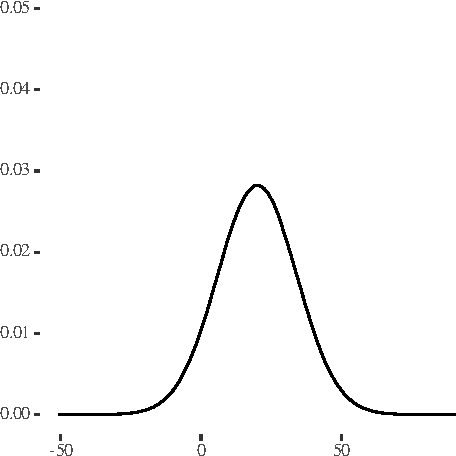
\includegraphics[width=0.4\linewidth]{AdditivityOfVariance4th_files/figure-latex/unnamed-chunk-9-1} }\subfloat[$df_1 = 9, df_2 = 3$\label{fig:unnamed-chunk-9-2}]{\includegraphics[width=0.4\linewidth]{AdditivityOfVariance4th_files/figure-latex/unnamed-chunk-9-2} }

}

\caption[分散を加算する二種類のF分布]{分散を加算する二種類のF分布}\label{fig:unnamed-chunk-9}
\end{figure}

\begin{table}

\caption{\label{tab:unnamed-chunk-11}計算結果}
\centering
\resizebox{\linewidth}{!}{
\begin{tabular}[t]{rrrrrrrrrr}
\toprule
No & 相関係数 & p値 & 標本x & 標本y & 加法1 & 加法2 & 差異 & 加法1/加法2 & cov2\\
\midrule
\cellcolor{gray!6}{1} & \cellcolor{gray!6}{0.0002393} & \cellcolor{gray!6}{0.5926248} & \cellcolor{gray!6}{5.283749} & \cellcolor{gray!6}{9299.3652} & \cellcolor{gray!6}{2326.1888} & \cellcolor{gray!6}{2326.1622} & \cellcolor{gray!6}{0.0265195} & \cellcolor{gray!6}{1.0000114} & \cellcolor{gray!6}{0.0265195}\\
2 & -0.0002609 & 0.5596816 & 5.140466 & 6937.4608 & 1735.6257 & 1735.6503 & -0.0246314 & 0.9999858 & -0.0246314\\
\cellcolor{gray!6}{3} & \cellcolor{gray!6}{-0.0005290} & \cellcolor{gray!6}{0.2368538} & \cellcolor{gray!6}{5.126077} & \cellcolor{gray!6}{1723.8906} & \cellcolor{gray!6}{432.2293} & \cellcolor{gray!6}{432.2542} & \cellcolor{gray!6}{-0.0248643} & \cellcolor{gray!6}{0.9999425} & \cellcolor{gray!6}{-0.0248643}\\
4 & 0.0001149 & 0.7971652 & 5.262574 & 1077.7077 & 270.7469 & 270.7426 & 0.0043281 & 1.0000160 & 0.0043281\\
\cellcolor{gray!6}{5} & \cellcolor{gray!6}{0.0001032} & \cellcolor{gray!6}{0.8175539} & \cellcolor{gray!6}{5.159225} & \cellcolor{gray!6}{1275.7443} & \cellcolor{gray!6}{320.2301} & \cellcolor{gray!6}{320.2259} & \cellcolor{gray!6}{0.0041850} & \cellcolor{gray!6}{1.0000131} & \cellcolor{gray!6}{0.0041850}\\
\addlinespace
6 & 0.0003099 & 0.4883332 & 5.203402 & 1559.4609 & 391.1800 & 391.1661 & 0.0139581 & 1.0000357 & 0.0139581\\
\cellcolor{gray!6}{7} & \cellcolor{gray!6}{0.0000123} & \cellcolor{gray!6}{0.9780831} & \cellcolor{gray!6}{5.103390} & \cellcolor{gray!6}{925.8786} & \cellcolor{gray!6}{232.7459} & \cellcolor{gray!6}{232.7455} & \cellcolor{gray!6}{0.0004223} & \cellcolor{gray!6}{1.0000018} & \cellcolor{gray!6}{0.0004223}\\
8 & 0.0002263 & 0.6127805 & 5.339981 & 964.3089 & 242.4203 & 242.4122 & 0.0081209 & 1.0000335 & 0.0081209\\
\cellcolor{gray!6}{9} & \cellcolor{gray!6}{0.0007682} & \cellcolor{gray!6}{0.0858299} & \cellcolor{gray!6}{5.211663} & \cellcolor{gray!6}{1180.5351} & \cellcolor{gray!6}{296.4668} & \cellcolor{gray!6}{296.4367} & \cellcolor{gray!6}{0.0301293} & \cellcolor{gray!6}{1.0001016} & \cellcolor{gray!6}{0.0301293}\\
10 & -0.0003568 & 0.4249735 & 5.127960 & 864.1476 & 217.3070 & 217.3189 & -0.0118757 & 0.9999454 & -0.0118757\\
\addlinespace
\cellcolor{gray!6}{11} & \cellcolor{gray!6}{-0.0001285} & \cellcolor{gray!6}{0.7738059} & \cellcolor{gray!6}{5.161446} & \cellcolor{gray!6}{3846.1338} & \cellcolor{gray!6}{962.8147} & \cellcolor{gray!6}{962.8238} & \cellcolor{gray!6}{-0.0090546} & \cellcolor{gray!6}{0.9999906} & \cellcolor{gray!6}{-0.0090546}\\
12 & 0.0000877 & 0.8445989 & 5.157615 & 1642.7133 & 411.9718 & 411.9677 & 0.0040344 & 1.0000098 & 0.0040344\\
\cellcolor{gray!6}{13} & \cellcolor{gray!6}{-0.0002277} & \cellcolor{gray!6}{0.6106733} & \cellcolor{gray!6}{5.171313} & \cellcolor{gray!6}{221321.9773} & \cellcolor{gray!6}{55331.6654} & \cellcolor{gray!6}{55331.7872} & \cellcolor{gray!6}{-0.1217900} & \cellcolor{gray!6}{0.9999978} & \cellcolor{gray!6}{-0.1217900}\\
14 & 0.0000624 & 0.8890394 & 5.350175 & 1236.1945 & 310.3887 & 310.3862 & 0.0025372 & 1.0000082 & 0.0025372\\
\cellcolor{gray!6}{15} & \cellcolor{gray!6}{0.0001417} & \cellcolor{gray!6}{0.7512863} & \cellcolor{gray!6}{5.163609} & \cellcolor{gray!6}{2524.0812} & \cellcolor{gray!6}{632.3193} & \cellcolor{gray!6}{632.3112} & \cellcolor{gray!6}{0.0080909} & \cellcolor{gray!6}{1.0000128} & \cellcolor{gray!6}{0.0080909}\\
\addlinespace
16 & 0.0004361 & 0.3294718 & 5.346270 & 2559.8011 & 641.3124 & 641.2868 & 0.0255093 & 1.0000398 & 0.0255093\\
\cellcolor{gray!6}{17} & \cellcolor{gray!6}{0.0001128} & \cellcolor{gray!6}{0.8009107} & \cellcolor{gray!6}{5.272119} & \cellcolor{gray!6}{12234.8436} & \cellcolor{gray!6}{3060.0432} & \cellcolor{gray!6}{3060.0289} & \cellcolor{gray!6}{0.0143208} & \cellcolor{gray!6}{1.0000047} & \cellcolor{gray!6}{0.0143208}\\
18 & 0.0003906 & 0.3824324 & 5.211134 & 3601.8563 & 901.7936 & 901.7669 & 0.0267571 & 1.0000297 & 0.0267571\\
\cellcolor{gray!6}{19} & \cellcolor{gray!6}{-0.0002745} & \cellcolor{gray!6}{0.5393874} & \cellcolor{gray!6}{5.508024} & \cellcolor{gray!6}{1170.0237} & \cellcolor{gray!6}{293.8719} & \cellcolor{gray!6}{293.8829} & \cellcolor{gray!6}{-0.0110170} & \cellcolor{gray!6}{0.9999625} & \cellcolor{gray!6}{-0.0110170}\\
20 & -0.0004689 & 0.2944065 & 5.239619 & 6599.0153 & 1651.0201 & 1651.0637 & -0.0435958 & 0.9999736 & -0.0435958\\
\bottomrule
\end{tabular}}
\end{table}

\bibliography{bib/references.bib}



\end{document}
